%package list
\documentclass{article}
\usepackage[top=3cm, bottom=3cm, outer=3cm, inner=3cm]{geometry}
\usepackage{multicol}
\usepackage{graphicx}
\usepackage{url}
%\usepackage{cite}
\usepackage{hyperref}
\usepackage{array}
%\usepackage{multicol}
\newcolumntype{x}[1]{>{\centering\arraybackslash\hspace{0pt}}p{#1}}
\usepackage{natbib}
\usepackage{pdfpages}
\usepackage{multirow}
\usepackage[normalem]{ulem}
\useunder{\uline}{\ul}{}
\usepackage{svg}
\usepackage{xcolor}
\usepackage{listings}
\lstdefinestyle{ascii-tree}{
    literate={├}{|}1 {─}{--}1 {└}{+}1 
  }
\lstset{basicstyle=\ttfamily,
  showstringspaces=false,
  commentstyle=\color{red},
  keywordstyle=\color{blue}
}
%\usepackage{booktabs}
\usepackage{caption}
\usepackage{subcaption}
\usepackage{float}
\usepackage{array}

\newcolumntype{M}[1]{>{\centering\arraybackslash}m{#1}}
\newcolumntype{N}{@{}m{0pt}@{}}


%%%%%%%%%%%%%%%%%%%%%%%%%%%%%%%%%%%%%%%%%%%%%%%%%%%%%%%%%%%%%%%%%%%%%%%%%%%%
%%%%%%%%%%%%%%%%%%%%%%%%%%%%%%%%%%%%%%%%%%%%%%%%%%%%%%%%%%%%%%%%%%%%%%%%%%%%
\newcommand{\itemEmail}{jperez@unsa.edu.pe}
\newcommand{\itemStudent}{García, Hidalgo, Huayhua, Jaita}
\newcommand{\itemCourse}{PW2}
\newcommand{\itemCourseCode}{1702122}
\newcommand{\itemSemester}{III}
\newcommand{\itemUniversity}{Universidad Nacional de San Agustín de Arequipa}
\newcommand{\itemFaculty}{Facultad de Ingeniería de Producción y Servicios}
\newcommand{\itemDepartment}{Departamento Académico de Ingeniería de Sistemas e Informática}
\newcommand{\itemSchool}{Escuela Profesional de Ingeniería de Sistemas}
\newcommand{\itemAcademic}{2023 - A}
\newcommand{\itemInput}{Del 05 Junio 2023}
\newcommand{\itemOutput}{Al 12 Junio 2023}
\newcommand{\itemPracticeNumber}{05}
\newcommand{\itemTheme}{Django Admin}
%%%%%%%%%%%%%%%%%%%%%%%%%%%%%%%%%%%%%%%%%%%%%%%%%%%%%%%%%%%%%%%%%%%%%%%%%%%%
%%%%%%%%%%%%%%%%%%%%%%%%%%%%%%%%%%%%%%%%%%%%%%%%%%%%%%%%%%%%%%%%%%%%%%%%%%%%

\usepackage[english,spanish]{babel}
\usepackage[utf8]{inputenc}
\AtBeginDocument{\selectlanguage{spanish}}
\renewcommand{\figurename}{Figura}
\renewcommand{\refname}{Referencias}
\renewcommand{\tablename}{Tabla} %esto no funciona cuando se usa babel
\AtBeginDocument{%
	\renewcommand\tablename{Tabla}
}

\usepackage{fancyhdr}
\pagestyle{fancy}
\fancyhf{}
\setlength{\headheight}{30pt}
\renewcommand{\headrulewidth}{1pt}
\renewcommand{\footrulewidth}{1pt}
\fancyhead[L]{\raisebox{-0.2\height}{
\includegraphics[width=3cm]{img/logo_episunsa.png}}}
\fancyhead[C]{\fontsize{7}{7}\selectfont	\itemUniversity \\ \itemFaculty \\ \itemDepartment \\ \itemSchool \\ \textbf{\itemCourse}}
\fancyhead[R]{\raisebox{-0.2\height}{
\includegraphics[width=1.2cm]{img/logo_abet}}}
\fancyfoot[L]{Estudiantes: García, Hidalgo, Huayhua, Jaita}
\fancyfoot[C]{\itemCourse}
\fancyfoot[R]{Página \thepage}

% para el codigo fuente
\usepackage{listings}
\usepackage{color, colortbl}
\definecolor{dkgreen}{rgb}{0,0.6,0}
\definecolor{gray}{rgb}{0.5,0.5,0.5}
\definecolor{mauve}{rgb}{0.58,0,0.82}
\definecolor{codebackground}{rgb}{0.95, 0.95, 0.92}
\definecolor{tablebackground}{rgb}{0.8, 0, 0}

\lstset{frame=tb,
	language=bash,
	aboveskip=3mm,
	belowskip=3mm,
	showstringspaces=false,
	columns=flexible,
	basicstyle={\small\ttfamily},
	numbers=none,
	numberstyle=\tiny\color{gray},
	keywordstyle=\color{blue},
	commentstyle=\color{dkgreen},
	stringstyle=\color{mauve},
	breaklines=true,
	breakatwhitespace=true,
	tabsize=3,
	backgroundcolor= \color{codebackground},
}

\begin{document}
	
	\vspace*{10px}
	
	\begin{center}	
		\fontsize{17}{17} \textbf{ Informe de Laboratorio \itemPracticeNumber}
	\end{center}
	\centerline{\textbf{\Large Tema: \itemTheme}}
	%\vspace*{0.5cm}	

	\begin{flushright}
		\begin{tabular}{|M{2.5cm}|N|}
			\hline 
			\rowcolor{tablebackground}
			\color{white} \textbf{Nota}  \\
			\hline 
			     \\[30pt]
			\hline 			
		\end{tabular}
	\end{flushright}	

	\begin{table}[H]
		\begin{tabular}{|x{4.7cm}|x{4.8cm}|x{4.8cm}|}
			\hline 
			\rowcolor{tablebackground}
			\color{white} \textbf{Estudiante} & \color{white}\textbf{Escuela}  & \color{white}\textbf{Asignatura}   \\
Garcia Valdivia, Ronald Pablo
           \begin{itemize}
               \item rgarciava@unsa.edu.pe
           \end{itemize}
Hidalgo Chinchay, Paulo Andre  
           \begin{itemize}
               \item phidalgo@unsa.edu.pe
           \end{itemize}
Huayhua Mayta, Iván Rodrigo
           \begin{itemize}
               \item  ihuayhuam@unsa.edu.pe
           \end{itemize}
Jaita Chura, José Manuel
           \begin{itemize}
               \item jjaitac@unsa.edu.pe 
           \end{itemize}
			 & \itemSchool & {\itemCourse \par Semestre: \itemSemester \par Código: \itemCourseCode}     \\
			\hline 			
		\end{tabular}
	\end{table}		
	
	\begin{table}[H]
		\begin{tabular}{|x{4.7cm}|x{4.8cm}|x{4.8cm}|}
			\hline 
			\rowcolor{tablebackground}
			\color{white}\textbf{Laboratorio} & \color{white}\textbf{Tema}  & \color{white}\textbf{Duración}   \\
			\hline 
			\itemPracticeNumber & \itemTheme & 04 horas   \\
			\hline 
		\end{tabular}
	\end{table}
	
	\begin{table}[H]
		\begin{tabular}{|x{4.7cm}|x{4.8cm}|x{4.8cm}|}
			\hline 
			\rowcolor{tablebackground}
			\color{white}\textbf{Semestre académico} & \color{white}\textbf{Fecha de inicio}  & \color{white}\textbf{Fecha de entrega}   \\
			\hline 
			\itemAcademic & \itemInput &  \itemOutput  \\
			\hline 
		\end{tabular}
	\end{table}
	
	\section{Competencias del curso}
	\begin{itemize}		
		\item General: C.c. Diseña responsablemente aplicaciones web, sus componentes o procesos para
            satisfacer necesidades dentro de restricciones realistas: económicas, medio ambientales, sociales,
            políticas, éticas, de salud, de seguridad, manufacturación y sostenibilidad.
		\item Específica: C.m. Construye responsablemente soluciones con tecnología web siguiendo un pro-
            ceso adecuado llevando a cabo las pruebas ajustada a los recursos disponibles del cliente.
		\item Específica: C.p. Aplica de forma flexible técnicas, métodos, principios, normas, estándares y
            herramientas del desarrollo web necesarias para la construcción de aplicaciones web e implemen-
            tación de estos sistemas en una organización.
	\end{itemize}
 
    \section{Resultado del estudiante}
    \begin{itemize}
        \item RE. 2 La capacidad de aplicar diseño de ingeniería para producir soluciones a problemas y diseñar
            sistemas, componentes o procesos para satisfacer necesidades específicas dentro de consideracio-
            nes realistas en los aspectos de salud pública, seguridad y bienestar; factores globales, culturales,
            sociales, económicos y ambientales.
        \item RE. 8 La capacidad de crear, seleccionar y utilizar técnicas, habilidades, recursos y herramientas
            modernas de ingeniería y tecnologías de la información, incluyendo la predicción y el modela-
            miento, con una comprensión de las limitaciones.
    \end{itemize}
		
	\section{Equipos, materiales y temas}
	\begin{itemize}
		\item Sistema Operativo (GNU/Linux de preferencia).
		\item GNU Vim.
		\item Python 3.
		\item Git.
		\item Cuenta en GitHub con el correo institucional.
		\item Entorno virtual.
		\item Django 4.	
	\end{itemize}
	
	\section{URL de Repositorio Github}
	\begin{itemize}
		\item URL del Repositorio GitHub para clonar o recuperar.
		\item \url{https://github.com/123ihuayhua/pweb2-lab-c-23a.git}
		\item URL para el laboratorio 05 en el Repositorio GitHub.
		\item \url{https://github.com/123ihuayhua/pweb2-lab-c-23a/tree/main/Lab5-Pweb2}
	\end{itemize}

    
    \section{Tarea}
    \begin{itemize}
        \item Elabore un primer informe grupal de la aplicación que desarrollará durante este semestre.
        \item Utilicen todas las recomendaciones dadas en la aplicación library.
        \item Acuerdos :
        \begin{itemize}
            \item Los grupos pueden estar conformado por 1 a 4 integrantes.
            \item Sólo se presenta un informe grupal.
            \item Sólo se revisa un repositorio. (El único que esté en el informe grupal).
            \item Todos los integrantes del grupo tienen una copia del laboratorio e informe en su repositorio privado.
            \item Todos los integrantes deben pertenecer al mismo grupo de laboratorio.
            \item El docente preguntará en cualquier momento a un integrante sobre el proyecto, codigo fuente, avance.
        \end{itemize}
    \end{itemize}

    \section{Pregunta}
    \begin{itemize}
        \item Por cada integrante del equipo, resalte un aprendizaje que adquirió al momento de estudiar
        Django. No se reprima de ser detallista. Coloque su nombre entre parentesis para saber que es
        su aporte.
        \item Django sigue el patrón de diseño MVC, lo que te permite organizar tu código de una manera estructurada y modular. (Hidalgo Chinchay, Paulo Andre)
        \item La ventaja de utilizar Django junto con el modelo entidad-relación es que puedes diseñar tu base de datos utilizando el modelo entidad-relación tradicional, y luego utilizar el ORM de Django para crear automáticamente la estructura de la base de datos y manipular los datos utilizando objetos de Python. El ORM se encarga de traducir las operaciones en objetos a consultas SQL que se ejecutan en la base de datos subyacente. (Huayhua Mayta, Iván Rodrigo) 
        \item En relación al modelo entidad-relación (MER), es un modelo conceptual utilizado en el diseño de bases de datos para representar y describir las entidades, atributos y relaciones entre ellas. El MER es independiente de cualquier implementación específica de base de datos, como MySQL o PostgreSQL. (Jaita Chura, José Manuel)
        \item La facilidad con la que es posible crear una base de datos gracias a Django, gracias a esto al conocer el lenguaje Python es más fácil el administar la base de datos. (Garcia Valdivia, Ronald Pablo) 
    \end{itemize}
    
    \section{Entregables}
    \begin{itemize}
        \item El informe debe tener un enlace al directorio específico del laboratorio en su repositorio GitHub
        privado donde esté todo el código fuente y otros que sean necesarios. Evitar la presencia de archi-
        vos: binarios, objetos, archivos temporales, cache, librerias, entornos virtuales. Si hay configura-
        ciones particulares puede incluir archivos de especificación como: requirements.txt, o leeme.txt.
        \item No olvide que el profesor debe ser siempre colaborador a su repositorio (Usuario del profesor
        @rescobedoq).
        \item Para ser considerado con la calificación de máxima nota, el informe debe estar elaborado en
        LATEX
        \item Usted debe describir sólo los commits más importantes que marcaron hitos en su trabajo,
        adjutando capturas de pantalla, del commit, del código fuente, de sus ejecuciones y pruebas.
        \item En el informe siempre se debe explicar las imágenes (codigo fuente, capturas de pantalla, commits,
        ejecuciones, pruebas, etc.) con descripciones puntuales pero precisas.
        \item Partes de entrega:
        \begin{itemize}
        
            \item Modelo de datos. (Diagrama Entidad-Relación)
            \begin{itemize}
                \item En el siguiente diagrama se muestran 6 clases: "Vendedor, Marcas, Artículo, Pedido Detalle, Pedido Cabecera y Cliente"
            \end{itemize}
            \begin{figure}[H]
		      \centering
                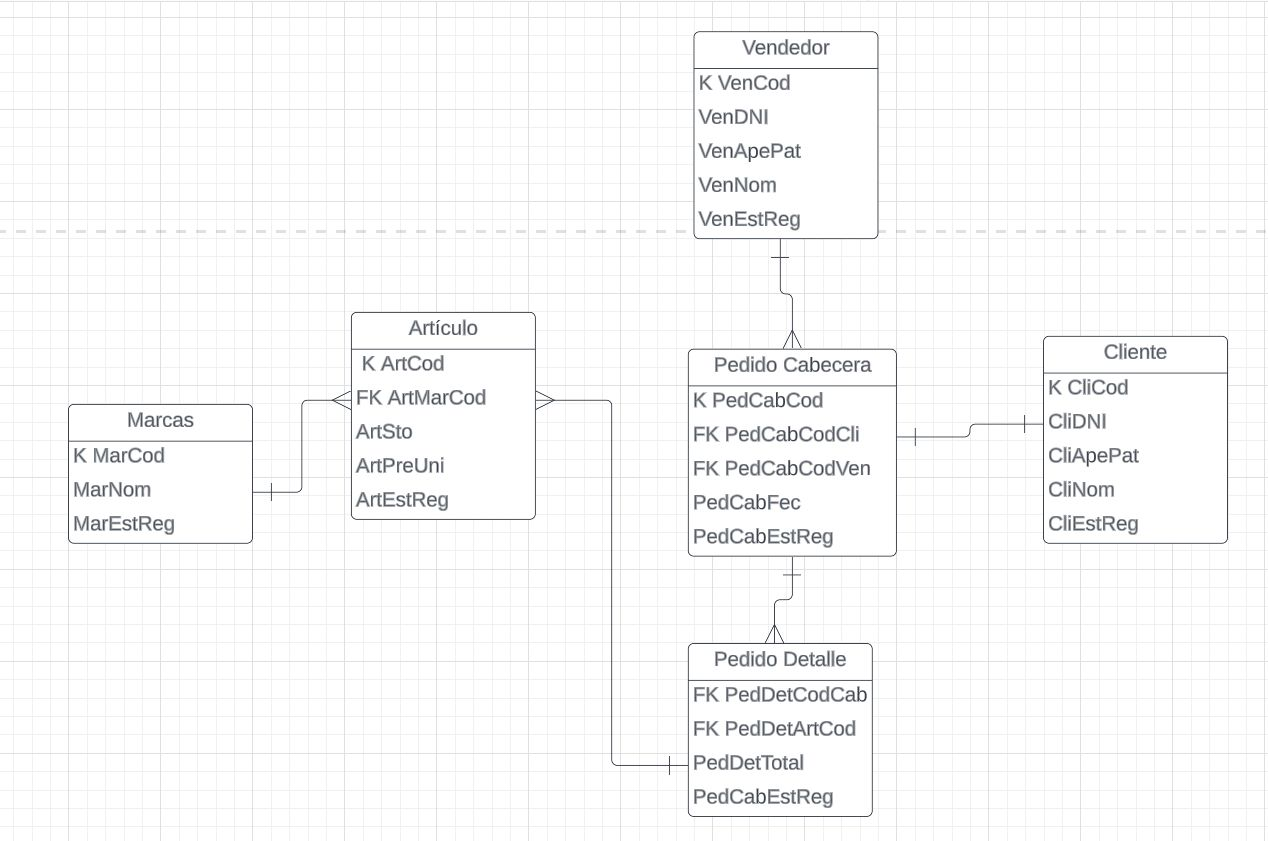
\includegraphics[width=0.8\textwidth,keepaspectratio]{img/Diagrama.jpeg}
		      %\includesvg{img/automata.svg}
		      %\label{img:mot2}
		      %\caption{Product backlog.}
	   \end{figure}
 
            \item Modelos Python.
            \begin{itemize}
                \item La clase "Vendedor" define un modelo de Django que representa a un vendedor en el sistema o aplicación que estás desarrollando.

                Este modelo tiene varios campos que representan diferentes atributos de un vendedor, como su DNI (Documento Nacional de Identidad), apellido paterno, nombre y estado de registro.
                \item El modelo "Cliente" hereda de la clase AbstractUser, que es una clase de modelo proporcionada por Django para la autenticación de usuarios. Esto significa que el modelo "Cliente" obtiene todos los campos y funcionalidades de AbstractUser, como nombre de usuario, contraseña, correo electrónico, etc.

                Además de los campos heredados, el modelo "Cliente" también tiene campos personalizados para representar atributos específicos del cliente, como su DNI, apellido paterno, nombre y estado de registro.
                
                \item Modelo marca: Este modelo permite almacenar información sobre diferentes marcas en tu sistema o aplicación.
                \item El modelo "TipoArticulo" define una entidad de tipo de artículo con dos campos:

                TipArtNom: Un campo de tipo CharField con una longitud máxima de 20 caracteres, que representa el nombre del tipo de artículo.
                TipArtEstReg: Un campo de tipo BooleanField que representa el estado de registro del tipo de artículo, con un valor predeterminado de True.
                Este modelo te permite almacenar información sobre diferentes tipos de artículos en tu sistema o aplicación.
                \item Clase "Articulo": Esta clase representa un artículo en el sistema o aplicación.
                Tiene los siguientes campos:
                ArtMarCod: Un campo de clave externa (ForeignKey) que referencia a la clase Marca y se utiliza para almacenar el código de marca del artículo.
                ArtTipCod: Un campo de clave externa (ForeignKey) que referencia a la clase TipoArticulo y se utiliza para almacenar el código de tipo de artículo.
                ArtNom: Un campo de tipo CharField con una longitud máxima de 50 caracteres, que representa el nombre del artículo.
                ArtDes: Un campo de tipo TextField que permite ingresar una descripción del artículo con un máximo de 1000 caracteres.
                ArtSto: Un campo de tipo IntegerField que representa el stock (cantidad disponible) del artículo.
                ArtPreUni: Un campo de tipo FloatField que representa el precio unitario del artículo.
                ArtEstReg: Un campo de tipo BooleanField que representa el estado de registro del artículo.
                Tiene una función str() que devuelve el nombre del artículo como representación legible cuando se convierte en una cadena.
                \item Clase "PedidoCabecera":Esta clase representa la cabecera de un pedido en el sistema o aplicación.
                Tiene los siguientes campos:
                PedCabCodCli: Un campo de clave externa (ForeignKey) que referencia a la clase Cliente y se utiliza para almacenar el código de cliente relacionado con el pedido.
                PedCabCodVen: Un campo de clave externa (ForeignKey) que referencia a la clase Vendedor y se utiliza para almacenar el código de vendedor relacionado con el pedido.
                PedCabFec: Un campo de tipo DateField que representa la fecha del pedido.
                PedCabEstReg: Un campo de tipo BooleanField que representa el estado de registro de la cabecera del pedido.
                Tiene una función str() que devuelve el código de cliente como representación legible cuando se convierte en una cadena.
                \item Clase "PedidoDetalle": Esta clase representa los detalles de un pedido en el sistema o aplicación.
                Tiene los siguientes campos:
                PedDetCodCab: Un campo de clave externa (ForeignKey) que referencia a la clase PedidoCabecera y se utiliza para almacenar el código de cabecera del pedido al que pertenece este detalle.
                PedDetArtCod: Un campo de clave externa (ForeignKey) que referencia a la clase Articulo y se utiliza para almacenar el código de artículo relacionado con este detalle.
                PedDetCantidad: Un campo de tipo IntegerField que representa la cantidad de artículos en este detalle del pedido.
                PedDetPreUniArt: Un campo de tipo FloatField que representa el precio unitario del artículo en este detalle del pedido.
                PedDetSubtotal: Un campo de tipo FloatField que representa el subtotal calculado para este detalle (cantidad * precio unitario).
                PedDetTot: Un campo de tipo FloatField que representa el total calculado para este detalle (igual al subtotal en este caso).
                PedDetEstReg: Un campo de tipo BooleanField que representa el estado de registro del detalle del pedido.
                Tiene una función save() personal.
            \end{itemize}
            \lstinputlisting[language=Python, caption={models.py},numbers=left,]{src/models.py}
            \begin{itemize}
                \begin{itemize}
                    \item admin.py muestra cómo personalizar la interfaz de administración de Django para los modelos Vendedor, Cliente y Articulo. Aquí hay una descripción de cada clase y su funcionalidad:
                    \item VendedorAdmin: Esta clase personaliza la interfaz de administración para el modelo Vendedor. Se define la variable list-display para especificar los campos que se mostrarán en la lista de registros de vendedores. Luego, se definen métodos para mostrar los valores de los campos personalizados en la lista. En este caso, se definen métodos como nombre, apellido y dni para mostrar los valores correspondientes de los campos del modelo Vendedor. También se proporcionan etiquetas personalizadas para los campos.
                    \item ClienteAdmin: Similar a VendedorAdmin, esta clase personaliza la interfaz de administración para el modelo Cliente. Se define list-display y métodos para mostrar los valores de los campos personalizados en la lista de registros de clientes.
                    \item ArticuloAdmin: Esta clase personaliza la interfaz de administración para el modelo Articulo. Se define list-display y métodos para mostrar los valores de los campos personalizados en la lista de registros de artículos. Además, se realiza un formato especial para el campo precio-unitario para mostrar el precio con un símbolo de moneda y formato decimal.
                    \item Luego, se registran las clases personalizadas en el administrador de Django utilizando admin.site.register para que las personalizaciones se apliquen a los modelos correspondientes.
                \end{itemize}
            \end{itemize}
            \lstinputlisting[language=Python, caption={admin.py},numbers=left,]{src/admin.py}

            \item Implementación del Django Administrador. (CRUD para todas las tablas)
            \begin{itemize}
                \item A continuación se muestran imágenes de la creación exitosa de la Base de datos.
            \end{itemize}
            \begin{figure}[H]
		      \centering
                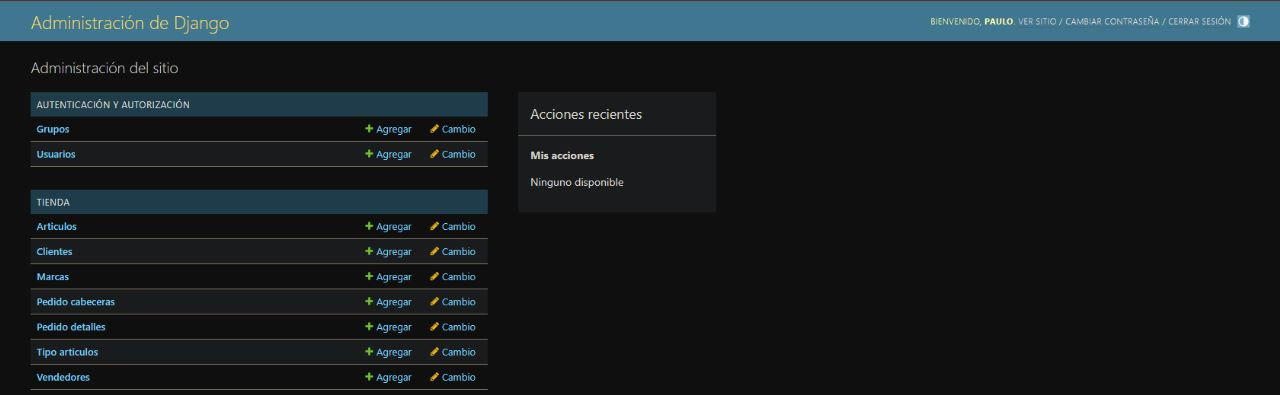
\includegraphics[width=0.8\textwidth,keepaspectratio]{img/V11.jpeg}
		      %\includesvg{img/automata.svg}
		      %\label{img:mot2}
		      \caption{Administración Django.}
	   \end{figure}
            \begin{figure}[H]
		      \centering
                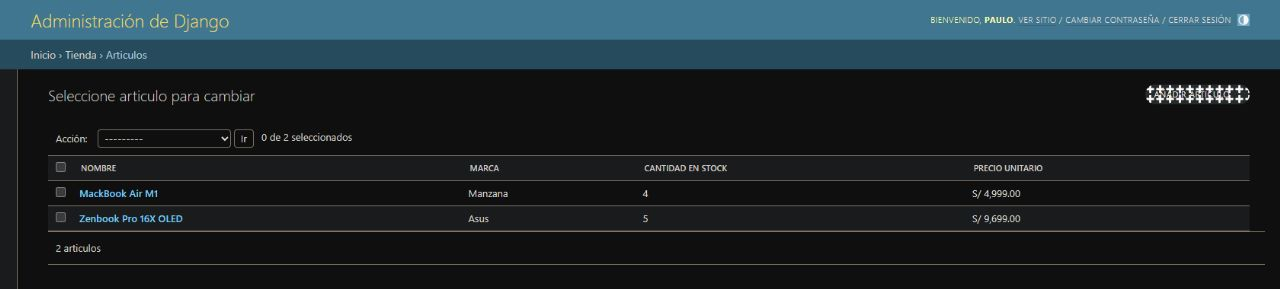
\includegraphics[width=0.8\textwidth,keepaspectratio]{img/V12.jpeg}
		      %\includesvg{img/automata.svg}
		      %\label{img:mot2}
		      \caption{Administración Django Artículos.}
	   \end{figure}
            \begin{figure}[H]
		      \centering
                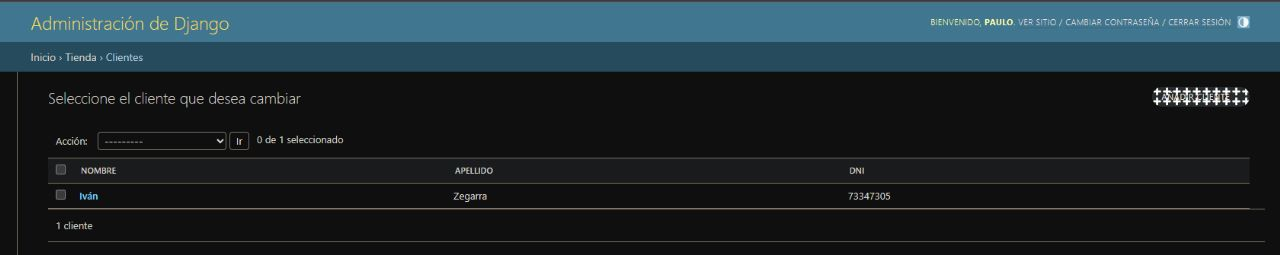
\includegraphics[width=0.8\textwidth,keepaspectratio]{img/V13.jpeg}
		      %\includesvg{img/automata.svg}
		      %\label{img:mot2}
		      \caption{Administración Django Clientes.}
	   \end{figure}
            \begin{figure}[H]
		      \centering
                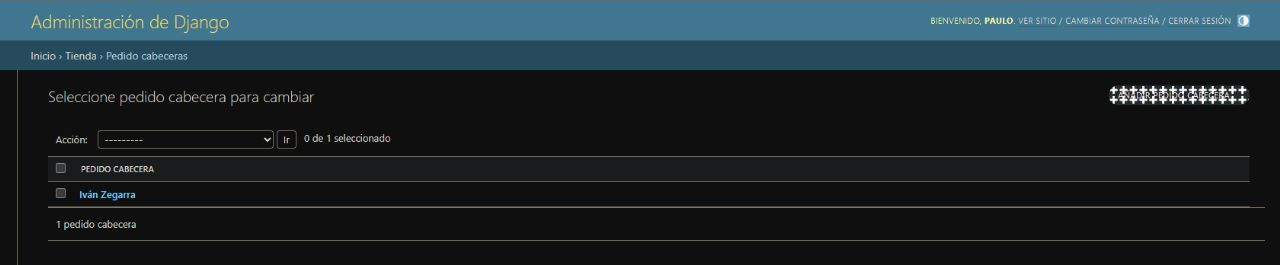
\includegraphics[width=0.8\textwidth,keepaspectratio]{img/V14.jpeg}
		      %\includesvg{img/automata.svg}
		      %\label{img:mot2}
		      \caption{Administración Django Pedido cabeceras.}
	   \end{figure}
            \begin{figure}[H]
		      \centering
                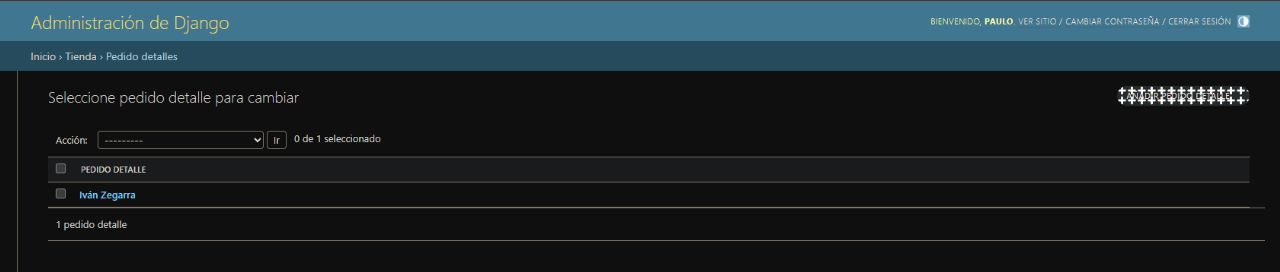
\includegraphics[width=0.8\textwidth,keepaspectratio]{img/V15.jpeg}
		      %\includesvg{img/automata.svg}
		      %\label{img:mot2}
		      \caption{Administración Django Pedido detalles.}
	   \end{figure}
            \begin{figure}[H]
		      \centering
                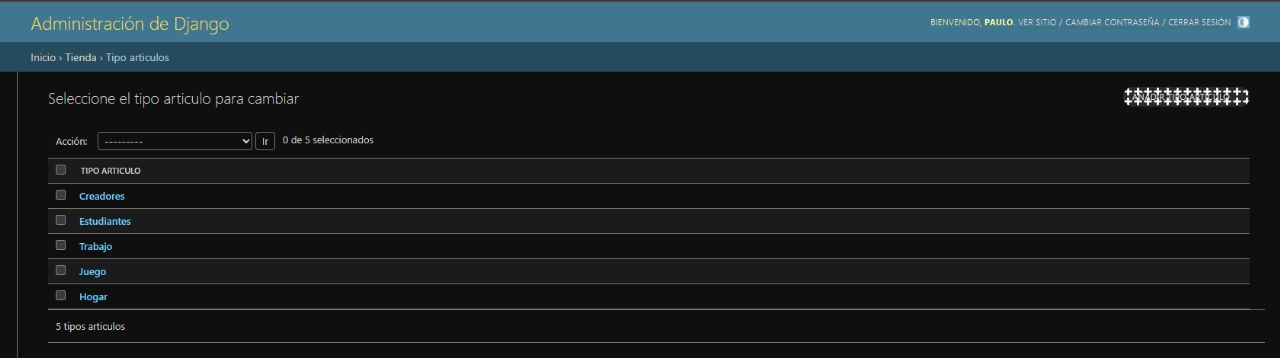
\includegraphics[width=0.8\textwidth,keepaspectratio]{img/V16.jpeg}
		      %\includesvg{img/automata.svg}
		      %\label{img:mot2}
		      \caption{Administración Django Tipo artículos.}
	   \end{figure}
            \begin{figure}[H]
		      \centering
                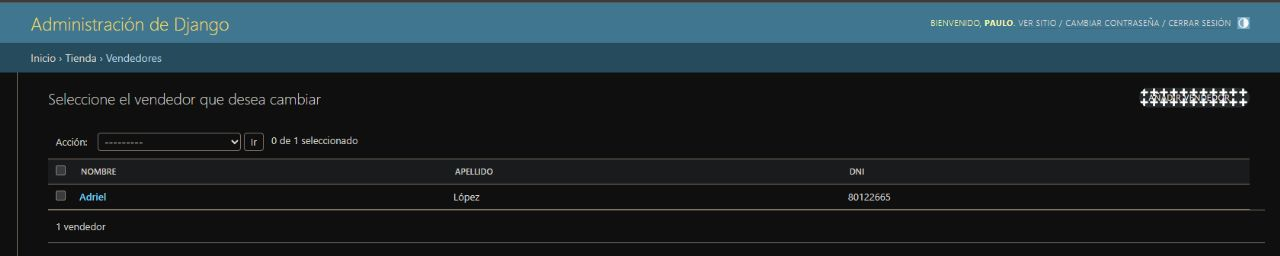
\includegraphics[width=0.8\textwidth,keepaspectratio]{img/V17.jpeg}
		      %\includesvg{img/automata.svg}
		      %\label{img:mot2}
		      \caption{Administración Django Vendedores.}
	   \end{figure}
            \item Considerar: atributos adecuados, relaciones necesarias, visualización de datos adecuadas,
            restricciones en el modelo importantes.
        \end{itemize}
    \end{itemize}

    \section{Commits}
    \begin{itemize}
        \item Los commits más importantes fueron los siguientes:
        \begin{itemize}
            \item Creación aplicación tienda: Es donde se crearán "views.py, models.py, forms.py, etc."
            \item Corrección a errores de migración, duplicación de modelos: Se elminaron las diferentes clases modelos que se había repartido etre lo miembros del equipo para juntarlas en una sola de manera funcional
            \item Modificación modelos y agregación de funciones: Se concretaron las funciones que nos permiten tener funciones en "Vendedor, Marcas, Artículo, Pedido Detalle, Pedido Cabecera y Cliente"
        \end{itemize}
        \item Todos commits realizados fueron los siguientes:
    \end{itemize}
    \begin{figure}[H]
		      \centering
                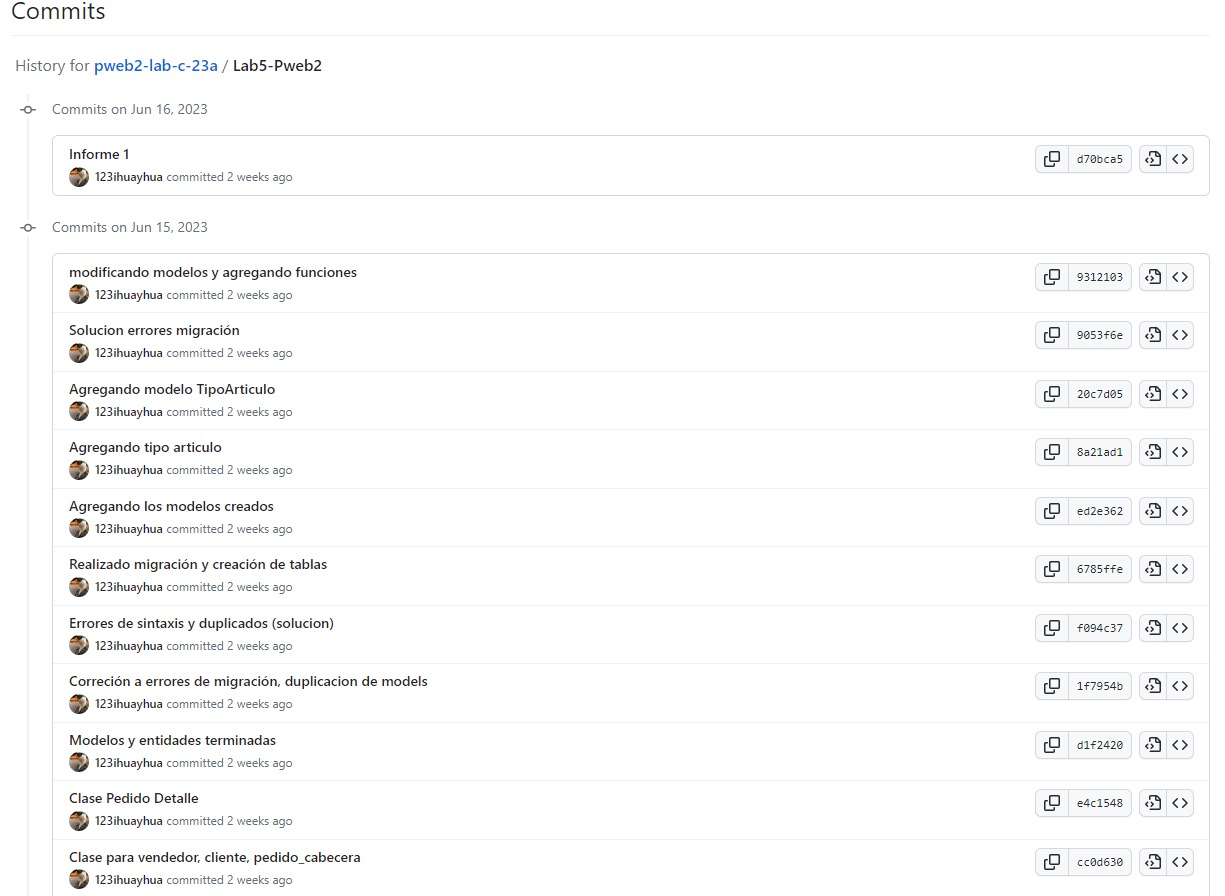
\includegraphics[width=0.8\textwidth,keepaspectratio]{img/C1.jpeg}
		      %\includesvg{img/automata.svg}
		      %\label{img:mot2}
		      %\caption{Product backlog.}
	   \end{figure}
    \begin{figure}[H]
		      \centering
                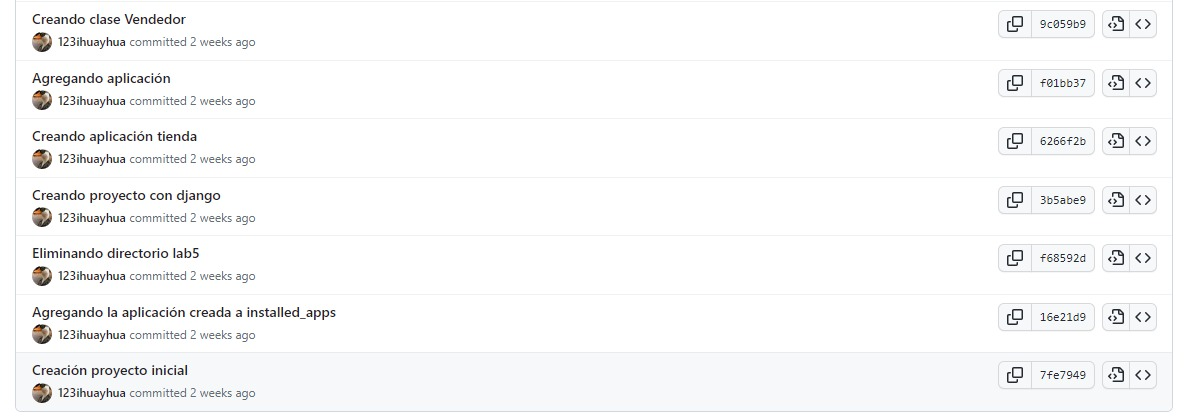
\includegraphics[width=0.8\textwidth,keepaspectratio]{img/C2.jpeg}
		    %\includesvg{img/automata.svg}
		    %\label{img:mot2}
		     %\caption{Product backlog.}
	\end{figure}
\clearpage
\section{Estructura del directorio}
\begin{document}
\begin{verbatim}
.
|-- db.sqlite3
|-- Latex-InformeLab05-Pweb
|   |-- img
|   |   |-- C1.jpeg
|   |   |-- C2.jpeg
|   |   |-- Diagrama.jpeg
|   |   |-- logo_abet.png
|   |   |-- logo_episunsa.png
|   |   |-- logo_unsa.jpg
|   |   |-- pseudocodigo_insercion.png
|   |   |-- V11.jpeg
|   |   |-- V12.jpeg
|   |   |-- V13.jpeg
|   |   |-- V14.jpeg
|   |   |-- V15.jpeg
|   |   |-- V16.jpeg
|   |   `-- V17.jpeg
|   |-- Lab05.pdf
|   |-- Lab05.pdf:Zone.Identifier
|   |-- Laboratorio05.tex
|   `-- src
|       |-- admin.py
|       |-- Insertion01.java
|       `-- models.py
|-- localstore
|   |-- asgi.py
|   |-- __init__.py
|   |-- __pycache__
|   |   |-- __init__.cpython-310.pyc
|   |   |-- settings.cpython-310.pyc
|   |   |-- urls.cpython-310.pyc
|   |   `-- wsgi.cpython-310.pyc
|   |-- settings.py
|   |-- urls.py
|   `-- wsgi.py
|-- manage.py
`-- tienda
    |-- admin.py
    |-- apps.py
    |-- __init__.py
    |-- migrations
    |   |-- 0001_initial.py
    |   |-- 0002_remove_articulo_artmarcod_articulo_artdes_and_more.py
    |   |-- 0003_remove_tipoarticulo_tipartcodmar.py
    |   |-- 0004_articulo_artmarcod.py
    |   |-- 0005_alter_pedidodetalle_peddetcodcab_and_more.py
    |   |-- 0006_pedidodetalle_peddetcantidad_and_more.py
    |   |-- 0007_remove_pedidodetalle_peddetprecio_and_more.py
    |   `-- __init__.py
    |-- models.py
    |-- __pycache__
    |   |-- admin.cpython-310.pyc
    |   |-- apps.cpython-310.pyc
    |   |-- __init__.cpython-310.pyc
    |   |-- models.cpython-310.pyc
    |   `-- views.cpython-310.pyc
    |-- tests.py
    `-- views.py

\end{verbatim}

	\section{\textcolor{red}{Rúbricas}}
	
	\subsection{\textcolor{red}{Entregable Informe}}
	\begin{table}[H]
		\caption{Tipo de Informe}
		\setlength{\tabcolsep}{0.5em} % for the horizontal padding
		{\renewcommand{\arraystretch}{1.5}% for the vertical padding
		\begin{tabular}{|p{3cm}|p{12cm}|}
			\hline
			\multicolumn{2}{|c|}{\textbf{\textcolor{red}{Informe}}}  \\
			\hline 
			\textbf{\textcolor{red}{Latex}} & \textcolor{blue}{El informe está en formato PDF desde Latex,  con un formato limpio (buena presentación) y facil de leer.}   \\ 
			\hline 
			
			
		\end{tabular}
	}
	\end{table}
	
	\clearpage
	
	\subsection{\textcolor{red}{Rúbrica para el contenido del Informe y demostración}}
	\begin{itemize}			
		\item El alumno debe marcar o dejar en blanco en celdas de la columna \textbf{Checklist} si cumplio con el ítem correspondiente.
		\item Si un alumno supera la fecha de entrega,  su calificación será sobre la nota mínima aprobada, siempre y cuando cumpla con todos lo items.
		\item El alumno debe autocalificarse en la columna \textbf{Estudiante} de acuerdo a la siguiente tabla:
	
		\begin{table}[ht]
			\caption{Niveles de desempeño}
			\begin{center}
			\begin{tabular}{ccccc}
    			\hline
    			 & \multicolumn{4}{c}{Nivel}\\
    			\cline{1-5}
    			\textbf{Puntos} & Insatisfactorio 25\%& En Proceso 50\% & Satisfactorio 75\% & Sobresaliente 100\%\\
    			\textbf{2.0}&0.5&1.0&1.5&2.0\\
    			\textbf{4.0}&1.0&2.0&3.0&4.0\\
    		\hline
			\end{tabular}
		\end{center}
	\end{table}	
	
	\end{itemize}
	
	\begin{table}[H]
		\caption{Rúbrica para contenido del Informe y demostración}
		\setlength{\tabcolsep}{0.5em} % for the horizontal padding
		{\renewcommand{\arraystretch}{1.5}% for the vertical padding
		%\begin{center}
		\begin{tabular}{|p{2.7cm}|p{7cm}|x{1.3cm}|p{1.2cm}|p{1.5cm}|p{1.1cm}|}
			\hline
    		\multicolumn{2}{|c|}{Contenido y demostración} & Puntos & Checklist & Estudiante & Profesor\\
			\hline
			\textbf{1. GitHub} & Hay enlace URL activo del directorio para el  laboratorio hacia su repositorio GitHub con código fuente terminado y fácil de revisar. &2 &X &2 & \\ 
			\hline
			\textbf{2. Commits} &  Hay capturas de pantalla de los commits más importantes con sus explicaciones detalladas. (El profesor puede preguntar para refrendar calificación). &4 &X &4 & \\ 
			\hline 
			\textbf{3. Código fuente} &  Hay porciones de código fuente importantes con numeración y explicaciones detalladas de sus funciones. &2 &X &2 & \\ 
			\hline 
			\textbf{4. Ejecución} & Se incluyen ejecuciones/pruebas del código fuente  explicadas gradualmente. &2 &X &2 & \\ 
			\hline			
			\textbf{5. Pregunta} & Se responde con completitud a la pregunta formulada en la tarea.  (El profesor puede preguntar para refrendar calificación).  &2 &X &2 & \\ 
			\hline	
			\textbf{6. Fechas} & Las fechas de modificación del código fuente estan dentro de los plazos de fecha de entrega establecidos. &2 &X &2 & \\ 
			\hline 
			\textbf{7. Ortografía} & El documento no muestra errores ortográficos. &2 &X &2 & \\ 
			\hline 
			\textbf{8. Madurez} & El Informe muestra de manera general una evolución de la madurez del código fuente,  explicaciones puntuales pero precisas y un acabado impecable.   (El profesor puede preguntar para refrendar calificación).  &4 &X &4 & \\ 
			\hline
			\multicolumn{2}{|c|}{\textbf{Total}} &20 & &20 & \\ 
			\hline
		\end{tabular}
		%\end{center}
		%\label{tab:multicol}
		}
	\end{table}
	
\clearpage

\section{Referencias}
\begin{itemize}			
    \item {https://developer.mozilla.org/en-US/docs/Learn/Server-side/Django/Tutorial_local_
library_website}
    \item \url{https://github.com/mdn/django-locallibrary-tutorial}
    \item \url{https://github.com/rescobedoq/pw2/tree/main/labs/lab05}
    \item William S. Vincent. (2022). Django for Beginners: Build websites with Python. Django 4.0.
leanpub.com. [URL]
    \item \url{https://docs.djangoproject.com/en/4.1/ref/models/fields/}
    \item \url{https://docs.djangoproject.com/en/4.0/topics/db/examples/many_to_many/}
    \item \url{https://docs.djangoproject.com/en/4.0/topics/db/examples/many_to_one/}
    \item \url{https://blog.hackajob.co/djangos-new-database-constraints/}
    \item \url{https://stackoverflow.com/questions/3330435/is-there-an-sqlite-equivalent-to-mysqls-describe-table}
    \item \url{https://docs.djangoproject.com/en/4.1/ref/validators/#how-validators-are-run}
    \item \url{https://docs.djangoproject.com/en/4.1/ref/models/instances/}
    \item \url{https://www.youtube.com/watch?v=rHux0gMZ3Eg}
    \item \url{https://www.youtube.com/watch?v=OTmQOjsl0eg}
    \item \url{https://tex.stackexchange.com/questions/34580/escape-character-in-latex}
    \item \url{https://www.sqlitetutorial.net/sqlite-show-tables/}
    \item \url{https://www.wplogout.com/export-database-diagrams-erd-from-django/}
\end{itemize}	
	
%\clearpage
%\bibliographystyle{apalike}
%\bibliographystyle{IEEEtranN}
%\bibliography{bibliography}
			
\end{document}